\section{Initial proof-of-concept realisation}  \label{eq:realisation}

%\note{PM: below are the spare bits of implementation that I removed from the first part}
%
%\authornote{During normal operation, the broker In our testbed we by extending a Mosquitto MQTT broker so it logs each message routing event as a tuple into a \textit{TrackerDB} database
%	$ \langle p_i, c_j, t_k \rangle $
%}
%
%\authornote{We use a Cassandra NoSQL database for the \textit{TrackerDB}, to ensure scalability. 
%	A traffic reporting service generates traffic cubes on demand by querying the \textit{TrackerDB}, in response to requests issued by client applications (including possibly independent third party clients). The service is accessible through a REST interface.}
%
%\authornote{In our testbed deployment we use MQTT brokers, and the gateways generate messages by encapsulating either a batch of the raw data stream or an aggregation of it, depending on the type of stream, into the MQTT payload.}
	
	
	


\subsection{Background concepts: Blockchain and Smart Contracts}  \label{sec:blockchain}
Blockchain is essentially a distributed ledger of information (e.g., a transaction from A to B in the bitcoin world), a copy of which cannot be arbitrarily altered without being spotted and for which consistency of each information can be achieved through a decentralized and distributed consensus, without requiring trust in any third party but instead, through large and flat pool of so-called miners using cryptographic primitives~\cite{nakamoto2008bitcoin}.
Blockchain has been later leveraged to manage Smart Contracts, small pieces of software that encode a set of conditions and actions that a machine can interpret and that can be executed as expected using the blockchain infrastructure without third party involvement or supervision~\cite{Buterin2014}. Smart contracts represent therefore a well-suited decentralized tool to implement cube consistency and settlement functionalities. Being one of the most adopted and well-supported by the developers community, we decide to use Ethereum Smart Contract implementation\footnote{https://www.ethereum.org}.

In the Ethereum network, any node uses a virtual machine (EVM), which can execute code of arbitrary algorithmic complexity, to execute smart contracts, the integrity of whose is always guaranteed. A smart contract can perform various state updates and account balancing.  
Executing a smart contract results in one or more transactions to be validated. Each transaction has a cost (e.g., fee) associated, which translates into incentive for any miner within the network to independently execute it. 
More specifically, any operation being performed within a transaction consumes a fixed amount of Gas. Miners fees are therefore proportional to the amount of Gas used. Gas price is measured in terms of Ether (the Ethereum cryptocurrency). Every transaction specifies the gas price a smart contract is willing to pay for its execution, thus, the total fees paid for a transaction is the result of Gas amount multiplied by the Gas selected price.

%The second element of our approach is based on the use of emergin Blockchain and Smart Contracts tecnhology.

%\note{FIXME -- still a dump of Michele's text . background}

%Blockchain is essentially a distributed ledger of information (e.g., a transaction from A to B in the bitcoin world), a copy of which cannot be arbitrarily altered without being spotted and for which consistency of each information can be achieved in a decentralized and distributed way, without requiring trust in any third party. These properties, that in the bitcoin world provides a very strong business case (e.g., removing transaction costs associated to clearinghouse functionalities when transferring money), can also provide a trust case for exchanging access to different assets, without requiring trust among parties.

%Decentralized Applications (DApps) use assets and services from different sources, not controlled by only one entity (in contrast to the traditional centralized client/server web). Using smart contracts and off-chain information makes more practical to develop new DApps. s-Health apps can be seen as a particular type of DApps. Bitcoin is the first DApp built on top of the blockchain: it is a digital and interoperable currency (i.e., it does not require conversion across the world), using the blockchain infrastructure and some complex cryptographic algorithms, to achieve (nearly) zero transaction fees while avoiding the double-spending problem (e.g., possibility to spend a given amount twice) and without requiring to trust in any third party to police this risk. Thinking about the value of different assets, bitcoin and alt-coin (i.e., bitcoin plus metadata) can provide an interoperable and open cross-domain incentives platform for redistributing the value created from assets sharing, transparently covering the interests of all the involved assets providers.

%Blockchain has been later leveraged to manage Smart Contracts, small pieces of software that encode a set of conditions and actions that a machine can interpret and that can be executed as expected using the blockchain infrastructure without third party involvement or supervision \cite{Buterin2014}. These functionalities can be interesting when it comes to give permission to access different assets (datasets and devices) only for specific purposes.

%Blockchain is usually adopted by Decentralized Autonomous Organizations (DAOs), which require neither written statements nor physical governance bodies, to run on code expressed by a set of Smart Contracts. This concept is interesting for organizations where different stakeholders can vote and agree on the rules for sharing their assets, e.g., for particular social benefits or research purpose, thus deciding how their rewards should be distributed while influencing and supporting the creation of specific s-Health services. Through DAOs, the principles, rules and benefits deriving from data sharing can be distributedly enforced without requiring any trusted third party. While this is a powerful concept to achieve autonomy and avoid misuse, particular attention is required in order to properly encode the right human assisted governance structure in the DAOs. This might require a governance body that supervises the rules implemented as DAO by an open developers community, following a rigorous, open, transparent and accounted review process.


%\note{ANDREA}


%\authornote{We need reference to ETH architecture, with APIs call and a snippet of the code. We can add some numbers on how much this will cost to run and consequently set up a minimum cost for each data in order to keep infrastructure sustainable.
%Logic: “data” is a “count cube”. The platform generates a stream of these cubes at a certain rate, which is tunable using the window size on the TrackerDB. The arrival rate of the cubes determines the frequency at which contracts are executed, and therefore the cost over time.
%}
\vspace{-10pt}
\subsection{Implementation}
\label{sec:implementation}
For the purpose of experimentation and evaluation, we have adapted the open-source Mosquitto MQTT broker to support message logging and cubes generation into a Cassandra NoSQL database. We refer to it as the \textit{TrackerDB}. We connected to the MQTT broker real producers using channels provided by the ThingSpeak platform\footnote{https://thingspeak.com}.
Using the TrackerDB, we are able to simulate the generation of unilateral cubes that can be either complete and correct, or reflect malicious behaviour, for evaluation purposes.
The TrackerDB can be queried by any third party client through a REST service interface. Smart Contracts interact with the service through an Ethereum-specific mechanism, described below. 
In reality, unilateral cubes would be generated by gateways on the producers side as well as by VAS within their Trusted Zones. This does not affect the properties of the cubes compliance and settlement, because liability is pushed at the edge.
%
%Section~\ref{sec:no-trust} provides some detail on how unilateral cube generation can be implemented. 
%by extending a Mosquitto MQTT broker so it logs each message routing event as a tuple into a \textit{TrackerDB} database $ \langle p_i, c_j, t_k \rangle $

We now focus on the use of smart contracts in this setting.  We developed them using Solidity, the Ethereum's scripting language. To implement the contracts we assigned an Ethereum account to each producer and VAS. We connected these accounts to our private Ethereum test network, deployed on a single node with 6-core Intel Xeon E5-2640 and 16GB of RAM. We wrote, deployed and evaluated smart contracts in the network by using the Ethereum web browser based IDE Remix, connected to our private chain through Remote Procedure Call (RPC) protocol. In our implementation, accounts prepare and send the transactions to the blockchain to instances of Geth\footnote{https://github.com/ethereum/go-ethereum/wiki } through RPC. To measure gas consumption, we used the debug tool provided by Remix and we observed the difference in the account balance before and after invoking a settlement contract.

A limitation of Ethereum smart contracts is that they cannot directly access off-chain data about real-world state and events. In our case this represents a challenge in acquiring unilateral cubes value. More precisely, smart contracts are independently executed by any node in the chain, thus, each execution needs to retrieve such information from an off-chain source independently, without any assurance on the information integrity.
To overcome this limit, the concept of \emph{oracle} has been introduced. Simply speaking, an oracle is a special contract that serves data requests from traditional contracts, by sourcing them from designated data feeds. 
Two options are possible for implementing oracles. The first one is relying on existing proxy services. Oraclize\footnote{http://www.oraclize.it} provides a \emph{programmable} oracle that can interact with any data source selected among a predefined set of standard channels. In addition Oraclize provides an authenticity proof by means of a TLSNotary proof which guarantees the authenticity and integrity of the retrieved data. These functionalities come at a cost. For each off-chain query, Oraclize requires a fee which includes a commission, ranging from 0.01\$ to 0.04\$, and a refund of the Gas used to perform the transaction. 
The other option is when each party of the contract, producer and VAS, independently update their view of unilateral cubes by pulling their values from cubes generator located within their Trusted Zones and then creating a transaction which embeds the cubes in the blockchain. This way any node executing the smart contract will have the same copy of that cube. As a result, costs associated to the use of an external oracle proxies, such as Oraclize, can be saved. Because in our model responsibility and liability of producing faulty cubes is placed to producers and VAS, this option well suffices to our needs.

Pseudocode~\ref{settlement_contract} shows pseudo-code of our settlement contract. For the sake of simplicity, this snippet of code only accounts for the single producer and the single VAS scenario, although generalisation are straightforward.
The contract first requests the involved parties to provide their unilateral cubes; then it uses this information to perform the actual settlement, by combining the two unilateral cubes. If the processed combined cube is consistent then a payment to the producer is performed, otherwise, a dispute resolution mechanism should be invoked\footnote{At this time, our implementation simply reports and log the detected inequalities}.
%
\begin{algorithm}
	\caption{Cube settlement contract}\label{settlement_contract}
\begin{algorithmic}
	\IF{sender $\neq$ authorizedAddress}
	\STATE throw
	\IF{queryId $=$ producerQuery}
	\STATE producer $\gets$ unilateralCube
	\STATE vasQuery $\gets$ update()
	\ELSIF{queryId $=$ vasQuery}
	\STATE vas $\gets$ unilateralCube
	\IF {producer $=$ vas}
	\STATE transfer(producerAccount, dataPrice, cube)
	\ELSE
	\STATE disputeResolution()
	\ENDIF
	\ENDIF
	\ENDIF
\end{algorithmic}
\end{algorithm}
%
When a dispute resolution is invoked, payments are retained from being performed due to impossibility to clearly identify the correct unilateral cube. However a reputation mechanism can be implemented in order to penalise both parties involved in a given settlement transaction and to ultimately promote honest behaviour. As it is not expected that reputation computation will require off-chain interactions~\cite{schaub2016trustless,carboni2015feedback}, we are confident that while not considering its implementation in this phase this will not significantly affect the overall contract execution cost.

Table~\ref{tab:execution_costl} shows the execution cost of cube settlement operations expressed in Gas without and with Oraclize respectively. The most expensive operation to be performed is the \emph{contract deployment}, consuming from 175000 Gas without Oraclize to 2061490 Gas with Oraclize. The difference between these values is due to the higher number of functionalities implemented within Oraclize's API that the contract has to deploy\footnote{It is worth noticing that most of such functionalities are not required in a distributed liability model as the one promoted in our architecture}. Both the \emph{update} and \emph{callback} operations have a higher cost due to the Oraclize's fee, whereas the \emph{transfer} operation has the same cost.

\begin{table}[]
	\centering
	\caption{Execution cost of cube settlment contract operations.}
	\label{tab:execution_costl}
	\tiny 
	\resizebox{.4\textwidth}{!}{%
		\begin{tabular}{l|l|l|}
			\cline{2-3}
			& \multicolumn{2}{c|}{\textbf{Gas used}} \\ \hline
			\multicolumn{1}{|l|}{\textbf{Operation}} & w/o Oraclize & w Oraclize \\ \hline
			\multicolumn{1}{|l|}{Contract deployment} & 175000 & 2061490 \\ \hline
			\multicolumn{1}{|l|}{Update} & 41000 & 120000 \\ \hline
			\multicolumn{1}{|l|}{Callback} & 23000 & 70000 \\ \hline
			\multicolumn{1}{|l|}{Transfer} & 21000 & 21000 \\ \hline
		\end{tabular}%
	}
\end{table}
\vspace{-10pt}

\section{Evaluation and Lessons learnt}
\label{sec:evaluation}
Aim of this section is to quantify the cost of the smart contract described above and the associated cube settlement operations. By considering the scenario in which one VAS consumes the data of one producer, we evaluate how the cost of performing such contract affects the data price when the number of data exchanged and the number of settlements transactions required changes. Considering different quantity of exchanged data reflect the different purpose of the exchange (event-based data rather than real-time series acquisition). Nevertheless the reason for considering a variation in the number of required settlement needs some clarification. The most natural strategy will be to perform the settlement at the end of each contractually agreed data exchange, however in the early stage of an hypothetical market place where new producers and VAS join without necessarily trusting each other nor having an already established reputation, two situations might occur:
\begin{itemize}
	\item Producers and VAS have low reputation hence their trust level is low and the risk of claiming wrong unilateral cubes high. In this case, by performing more than one cube settlement, in an initial rump-up phase of a given data exchange will allow them to mutually increase their reputation and trust;
	\vspace{-10pt}
	\item Producers and VAS have already high reputation hence they are expected to act honestly. In this case cube settlements may occur with a lower rate, eventually only at the end of a data exchange phase, because the risk of producing faulty cubes is mitigated.
\end{itemize}
%1- 
%2- 

By evaluating the cost of performing the settlement operations we are able to define the minimum price that VAS should pay for each consumed data in order to sustain the settlement infrastructure and eventually generate profit for the producers.

We define the minimum data price as the amount of Ether needed to at least cover the cost of contract deployment and transactions for performing cubes settlement operations. This means that if a producer sells data at the minimum price, its profit will be zero. 
At the time of writing one Ether costs 220\$, however, its price is still very volatile (\url{etherscan.io/chart/etherprice}).

As result, transaction cost may frequently vary, thus leading to uncertainty about the economic feasibility of a specific application. We analysed the capability of Ethereum to support a stable transaction cost by tuning the Gas price. The main drawback when setting a low gas price is the increase of time required before a transaction is validated. Assuming a range of gas price between 0.9 Gwei and 20 Gwei (9e-10 and 2e-8 Ether respectively), as minimum and average reported by the Ethereum network in 2017, the time required for a transaction to be validated in the chain varies from 2 minutes to 14 seconds (\url{etherscan.io/chart}). As explained before, even in the case of multiple settlements, we do not expect that meaningful data exchange will last less than 2 minutes, thus we consider a viable choice to select the current minimum Gas price.


Figure~\ref{fig:overall} shows a general overview of the minimum data price by varying the frequency of cubes clearance operations and the amount of transferred data. The price is directly proportional to the increase of the number of cubes settlement performed while inversely proportional to the increase of data amount exchanged. Clearly, the more the data a VAS purchases, the less impacts the cost of performing cubes settlement. Depending on the type of data exchanged and trustworthiness of involved parties using this figure clearly shows how an optimal settlement strategy can always be found to dynamically adapt the number of settlement operations.

\begin{figure*}[t]
	\centering
	\subfigure[Minimum data price]{
		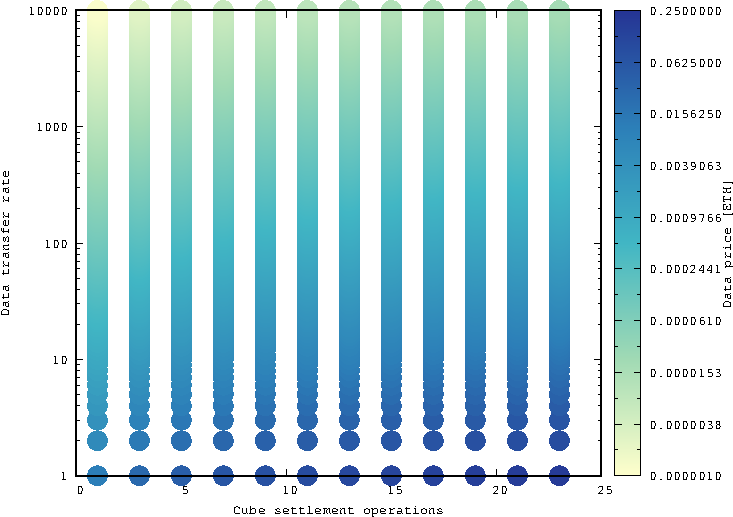
\includegraphics[width=.31\textwidth]{figures/feeNew-crop}
		\label{fig:overall}
	}%
	\subfigure[Cost without Oraclize]{
		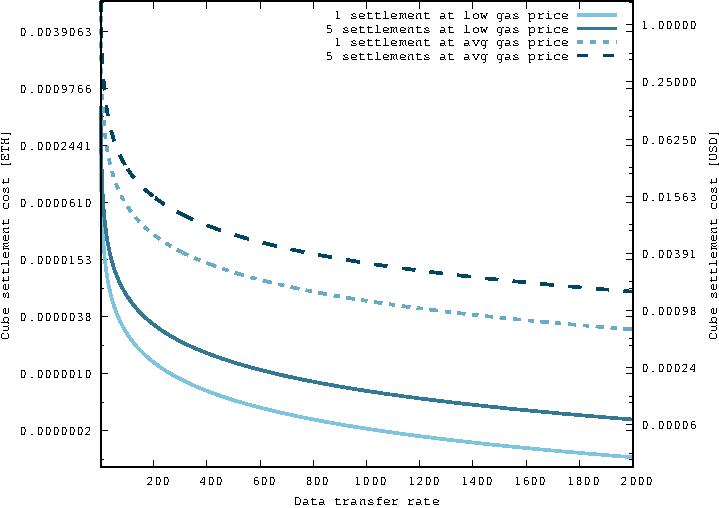
\includegraphics[width=.31\textwidth]{figures/resultSimple2-crop}
		\label{fig:noOraclize}
	}%
	\subfigure[Cost with Oraclize]{
		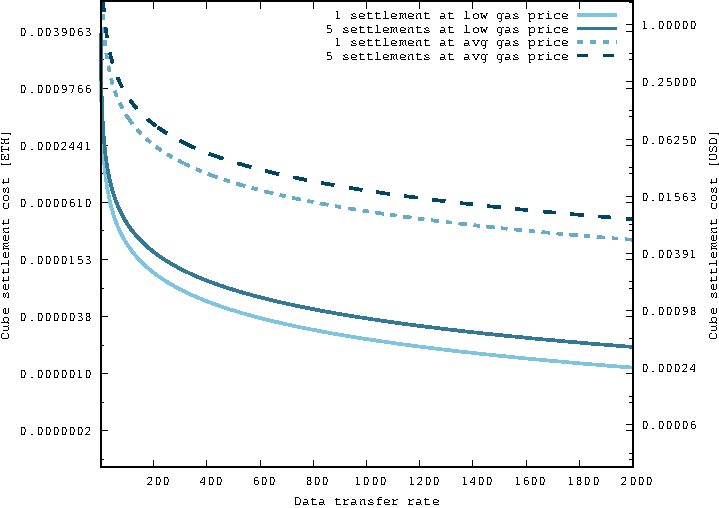
\includegraphics[width=.31\textwidth]{figures/resultOraclize2-crop}
		\label{fig:withOraclize}
	}%
	\caption{Cost of performing cube settlement operations for different data transfer rate.}
	\label{fig:all}
\end{figure*}

Figures~\ref{fig:noOraclize} and~\ref{fig:withOraclize} show the total cost of performing 1 or 5 cubes settlement operations for a fixed amount of transferred data, when considering a gas price ranging from 0.9 Gwei to 20 Gwei.
More specifically, figure~\ref{fig:noOraclize} shows the case when each party of the contract use its oracle implementation, while figure~\ref{fig:withOraclize} shows the case when Oraclize functionalities are used. 
It is worth noticing the large costs increase (on average 4 times more), due to the commission and refund of the Gas used to perform the transaction to be paid to Oraclize. 
Without Oraclize, the cost of a single cube settlement transaction ranges from 9.9e-5 (\$ 2.18e-2) Ether to 2.2e-3 Ether (\$ 4.84e-1) when the gas price selected is 0.9 Gwei and 20 Gwei respectively. The more amount of data is transferred, the less impact the transaction cost has per single data. In fact, when performing a cube settlement operation spread over 2000 data, its cost ranges from 1.26e-7 Ether (\$ 2.77e-5) to 2.8e-6 Ether (\$ 6.16e-4). Alternatively, when performing 5 cube settlement over 2000 data, their cost ranges from 3.15e-7 Ether (\$ 6.93e-5) to 7e-6 Ether (\$ 1.54e-3).
%1.26e-07	3.15e-07	2.8e-06	7e-06
When using Oraclize, the cost of a single cube settlement transaction ranges from 3.61e-4 Ether (\$ 7.94e-2) to 8.02e-3 Ether (\$ 1.76) when the gas price selected is 0.9 Gwei and 20 Gwei respectively. When performing a cube settlement operation spread over 2000 data, its cost ranges from 1.11e-6 Ether (\$ 2.44e-4) to 2.46e-5 Ether (\$ 5.42e-3). Alternatively, when performing 5 cube settlement over the same amount of data, their cost ranges from 1.83e-6 Ether (\$ 4.03e-4) to 4.07e-5 Ether (\$ 8.95e-3).
%\note{Add oraclize graph description}
%1.1081205e-06	1.8299205e-06	2.46249e-05	4.06649e-05
\begin{table}[!htp]
	\centering
	\caption{Estimated data price for different use cases.}
	\resizebox{.4\textwidth}{!}{%
		\begin{tabular}{r|c|r|r|r|}
			\cline{2-5}
			\multicolumn{1}{l|}{} & \multicolumn{4}{c|}{\textbf{Data price}} \\ \cline{2-5} 
			\multicolumn{1}{l|}{} & \multicolumn{2}{c|}{w/o Oraclize} & \multicolumn{2}{c|}{w Oraclize} \\ \hline
			\multicolumn{1}{|c|}{\textbf{Data rate}} & ETH & \multicolumn{1}{c|}{USD} & \multicolumn{1}{c|}{ETH} & \multicolumn{1}{c|}{USD} \\ \hline
			\multicolumn{1}{|r|}{high} & \multicolumn{1}{r|}{5.73e-8} & 1.26e-5 & 2.09e-7 & 4.59e-5 \\ \hline
			\multicolumn{1}{|r|}{medium} & \multicolumn{1}{r|}{3.44e-6} & 7.56e-4 & 1.25e-5 & 2.76e-3 \\ \hline
			\multicolumn{1}{|r|}{low} & \multicolumn{1}{r|}{2.06e-4} & 4.54e-2 & 7.52e-4 & 1.65e-1 \\ \hline
		\end{tabular}%
	}
	\label{tab:data_price}
\end{table}

In order to derive a profitable data price, we can assume that the cost of performing settlement operations has to be equal to 2\% of the price for that data amount and that only 1 cube settlement is performed per day. We consider two examples: 1) an air quality monitoring application, with low data rate, running on a Low Power Wide Area Network (LPWAN), such as Lora, that generates data every hour, resulting in 24 measurements per day; 2) a heart rate monitoring application (e.g., Fitbit), with sampling frequency of 1 second and 1 minute corresponding to a high and medium data rate respectively.  
Table~\ref{tab:data_price} shows that data price ranges from 5.73e-8 Ether (\$ 1.26e-5) to 7.52e-4 Ether (\$ 0.165) depending on data transfer rate and on the data feed type selected. 
%More specifically, Table~\ref{tab:data_price} shows estimated data price for different use cases, such as a heart rate monitoring application (e.g., fitbit), with sampling frequency of 1 second (high data rate), 1 minute (medium data rate) and 1 hour (low data rate).   

\subsection{Discussion}
\label{sec:discussion}
The analysis above helped us to identify the feasibility of building a decentralised open and transparent accounting infrastructure, useful to create a fair data marketplace, where data price can evolve depending on data quality, demand and offer. To minimise the shared costs of running such an infrastructure, we observed how the Gas price can be tweaked at the cost of a lower transaction rate, leveraging the lack of real-time requirements for the settlement operations. Moreover we demonstrated how the cubes architecture allow for scalability by reducing the settlement transaction frequency.
Nevertheless, we recognise that the estimated infrastructure costs are related to the current inflation in the Ether value, due to the large number of currently deployed general purpose smart contracts (raising up the Ether price of over 20 times in just one year). While we plan to perform similar analysis using different blockchain implementations like hyperledger (\url{hyperledger.org}), we anticipate that a decentralised marketplace will require to fork a new dedicated Ethereum network, dedicated to contract settlement, with lower incentive fees for the miners. While keeping it open, we are confident that, due to the large amount of IoT data exchanges such a market will support, a viable business opportunity for miners will still exist even at lower transaction and incentive fees.

%\authornote{
%\note{new from Michele}
%
%	\begin{itemize}
%\item test assuming no need of settlement, value are the same
%\item Test different time periods for cube generation, fine grained vs to larger interval, up to daily
%\item Invariance wrt to period for cube computation 
%\item Dependency wrt to number of sources and VAS (not addressed here)
%	\end{itemize}
%}
%
%
%\authornote{
%\note{old list}
%	\begin{itemize}
%		\item Are smart contracts an adequate implementation model to realise a fair marketplace?
%\item Are there limitations in the reconciliation phase?
%\item Cost of operating and marketplace: executing transactions and how to control them -- contract activated in an adaptive mode.  Who owns the contracts?  (ideal answer: nobody. Participants share the cost of transactions)
%\item Scalability: how the cubes decouple the data flow rates from the transaction frequency
%\item Data marketplace model is preliminary and not validated on real world use cases. It is based on minimal data semantics (ie the topic) and has no notion of more sophisticated contract models.
%	\end{itemize}
%}
%
%
%\authornote{
%\note{lessons learnt}
%
%	\begin{itemize}
%\item event vs time series, costs and requirements
%\item Liability of oracolize model for trust; requirements of new interfaces
%\item Volatility of market and price
%	\end{itemize}
%}
